\documentclass[a4paper,12pt]{article}
\usepackage[utf8]{inputenc}
\usepackage[spanish]{babel}
\usepackage{graphicx}
\usepackage{hyperref}
\usepackage{geometry}
\usepackage{longtable}
\usepackage{amsmath}
\usepackage{listings}
\usepackage{xcolor}
\usepackage{fancyhdr}
\usepackage{titlesec}
\usepackage{array}
\usepackage{booktabs}
\usepackage{float}

% Configuración de márgenes
\geometry{top=2.5cm, bottom=2.5cm, left=2.5cm, right=2.5cm}

% Configuración de encabezado y pie de página
\pagestyle{fancy}
\fancyhead{}
\fancyfoot{}
\fancyhead[L]{Un problema de reparacion.}
\fancyfoot[C]{\thepage}

% Configuración de títulos

\titleformat{\section}{\large\bfseries}{\thesection}{1em}{}
\titleformat{\subsection}{\normalsize\bfseries}{\thesubsection}{1em}{}
\titleformat{\subsubsection}{\normalsize\itshape}{\thesubsubsection}{1em}{}

% Configuración de código fuente
\lstset{
	basicstyle=\ttfamily\footnotesize,
	breaklines=true,
	commentstyle=\color{gray},
	keywordstyle=\color{blue},
	stringstyle=\color{red},
	numbers=left,
	numberstyle=\tiny\color{gray}
}

\begin{document}
	
	\begin{titlepage}
		\centering
		\vspace{1in}
		{\Huge \bfseries Un problema de reparación.  \par}
		\vspace{1.5in}
		\centering
		\vspace{1in}
		{\Huge \bfseries Autor \par}
		{\Large Victor Hugo Pacheco Fonseca  \par}
		
		\vfill
		{\Large \today \par}
	\end{titlepage}
	
	\tableofcontents
	\newpage
	
	\section{Introducción}
		\subsection{Descripcion del problema}
		Un sistema necesita n máquinas en funcionamiento para estar operativo. Para protegerse contra averías de la máquina, se mantienen disponibles máquinas adicionales como repuestos. Cada vez que una máquina se descompone, se reemplaza inmediatamente por una de repuesto y se envía al centro de reparación, que consta de un solo reparador que repara las máquinas averiadas una a la vez. Una vez que se ha reparado una máquina averiada, queda disponible como repuesto para ser utilizada cuando surja la necesidad.Ademas cada maquina produce una ganancia fija Q en una unidad de tiempo y cada reparacion tiene un costo fijo.
		En este proyecto se implementa una simulación de dicho proceso.
		
		\subsection{Objetivos}
		El objetivo principal se trata de determinar, mediante simulación, el tiempo promedio que transcurre hasta que ocurre una falla crítica (es decir, cuando una máquina falla y no quedan repuestos disponibles). Esto te permite evaluar la confiabilidad general del sistema y su capacidad operativa en función de los parámetros definidos.Ademas de verificar si existe un optimo en la cantidad de maquinas de respuestos para obtener la mayor ganancia.
		
		\subsection{Variables que describen el sistema}
		\subsubsection{Variables de tiempo}
		\begin{itemize}
			\item t: Tiempo total transcurrido.
			\item $t_i$: Tiempo de fallo de la maquina i.
			\item $t_*$: Tiempo de reparacion de la maquina que se encuentra en el taller.
			
		\end{itemize}
		\subsubsection{Variables de estado}
		\begin{itemize}
			\item r: Numero de maquinas que no se encuentran en funcionamiento.
			\item r: Ganancia total en un tiempo dado.
		\end{itemize}
	
	\section{Detalles de implentacion}
	  Todos los tiempos de reparación son variables aleatorias independientes que tienen la función de distribución Gamma con parametros alpha=1 ,beta=3.Cada vez que una máquina se pone en uso, la cantidad de tiempo que funciona antes de averiarse es una variable aleatoria, independiente del pasado, que tiene una función de distribución Gamma con parametros alpha=10,beta=30. Los valores de Q (ganancia por maquina) y de reparacion son constantes.
	
			\subsection{Inicio de la Simulación}
			Se utiliza el tiempo hasta la falla de la primera máquina en operación.Cuando esa máquina falla, se envía inmediatamente al taller de reparación y se utiliza una máquina de repuesto para mantener el sistema operativo.
			\subsection{Gestión de Fallas y Reparaciones}
			Después del primer evento, se compara el tiempo de falla de la siguiente máquina en operación con el tiempo de reparación de la máquina que se encuentra actualmente en el taller.
			\newline
			Si la próxima falla ocurre antes de que se complete la reparación:
			\begin{itemize}
				\item La máquina que falla se envía a la cola del taller.
				\item Se actualiza la ganancia obtenida hasta el tiempo actual.
				\item Se verifica si existe un repuesto disponible para sustituirla; de no haber repuesto, el sistema se bloquea y la simulación termina.
			\end{itemize}
			Si se completa la reparación antes de que ocurra la siguiente falla:
			\begin{itemize}
				\item La máquina reparada regresa y se añade al inventario de repuestos, quedándose disponible para reemplazar futuras fallas.
				\item Se actualiza la ganancia obtenida restando el costo de reparacion.
				\item Si hay otra máquina averiada pendiente, se inicia su reparación inmediatamente.
			\end{itemize}
			\subsection{Criterio de Parada}
			La simulación finaliza cuando ocurre una falla y ya no hay máquinas de repuesto disponibles para sustituir la máquina que acaba de fallar, y se retorna el tiempo final.
			
	\section{Resultados}
	Se realizaron 2 hipotesis basada en los datos obtenidos de la simulacion.
		
		\subsection{Hipótesis 1:Impacto del Número de Repuestos en el Tiempo hasta Bloqueo}
		
			Esta hipótesis se formulo considerando que, en un sistema en el que se tiene un número fijo de máquinas en operación, disponer de repuestos adicionales permite reemplazar las máquinas que fallan y, por ende, prolongar el tiempo en que el sistema opera antes de quedar bloqueado. Se espera que al aumentar el número de repuestos (designado como s), el tiempo promedio hasta el bloqueo, M, se incremente.
			\newline
			\newline
			
			Resultados Experimentales: En los experimentos se simuló el sistema fijando, por ejemplo,  máquinas en operación (n=100) y variando s
			de 1 a 80. La siguiente figura muestra los resutados optenidos:
			\begin{figure}[H]
				\centering
				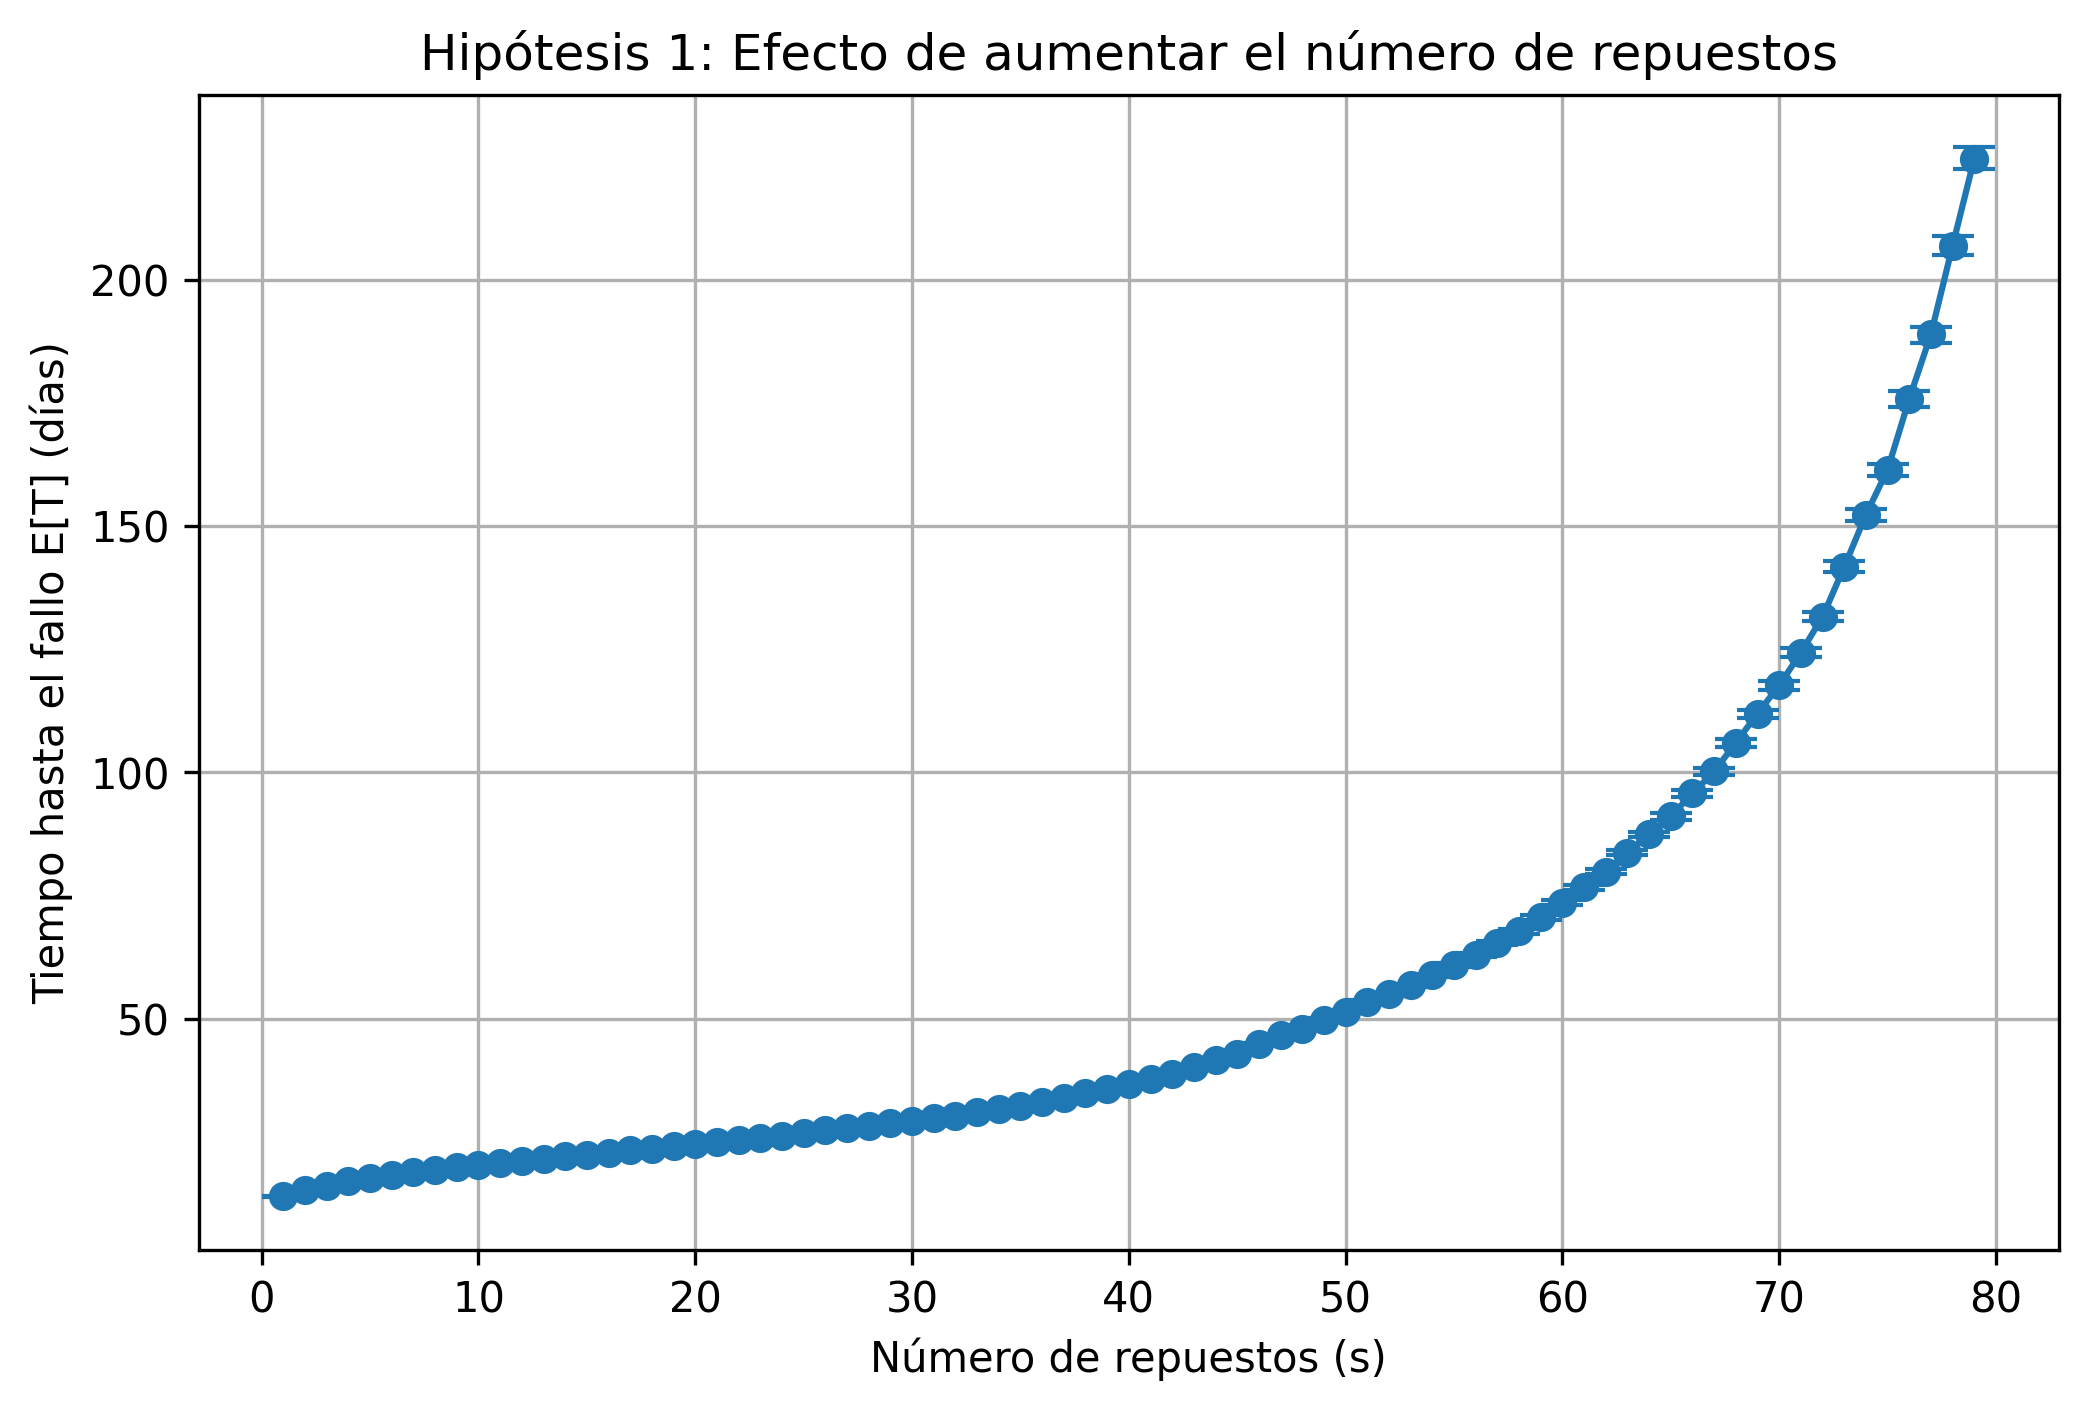
\includegraphics[width=\textwidth]{figure1.png}
				\caption{Tiempo de fallo Vs Numero de respuestos}
				\label{fig:Tiempo de fallo Vs Numero de respuestos}
			\end{figure}
			
		La evidencia experimental respalda esta hipótesis. Se acepta que aumentar el número de repuestos alarga la vida operativa del sistema.
			
		\subsection{Hipótesis 2: Ganancia Neta Acumulada versus Número de Repuestos}
		Esta hipótesis se basa en que la ganancia neta del sistema—definida como los ingresos generados por las máquinas en operación (a una tasa 
		Q
		por unidad de tiempo) menos el costo fijo que se incurre por cada reparación—depende de la cantidad de repuestos disponibles. Se espera que, al disponer de más repuestos, el sistema pueda operar por períodos más largos, lo que aumenta los ingresos. Pero cada repuesto adicional también puede implicar un mayor número de reparaciones, lo cual incrementa los costos. Por ello, existe la expectativa de que la ganancia neta aumente al aumentar s
		hasta alcanzar un óptimo; más allá de ese punto, el efecto de los costos de reparación podría contrarrestar los beneficios adicionales, e incluso la ganancia neta podría estabilizarse o decrecer.
		\newline
		\newline
		
		Resultados Experimentales: En los experimentos se simuló el sistema fijando, por ejemplo,  máquinas en operación (n=100) y variando s
		de 10 a 90,aplicando Q=1 y un costo de reparacion de 16 unidades. La siguiente figura muestra los resutados optenidos:
		\begin{figure}[H]
			\centering
			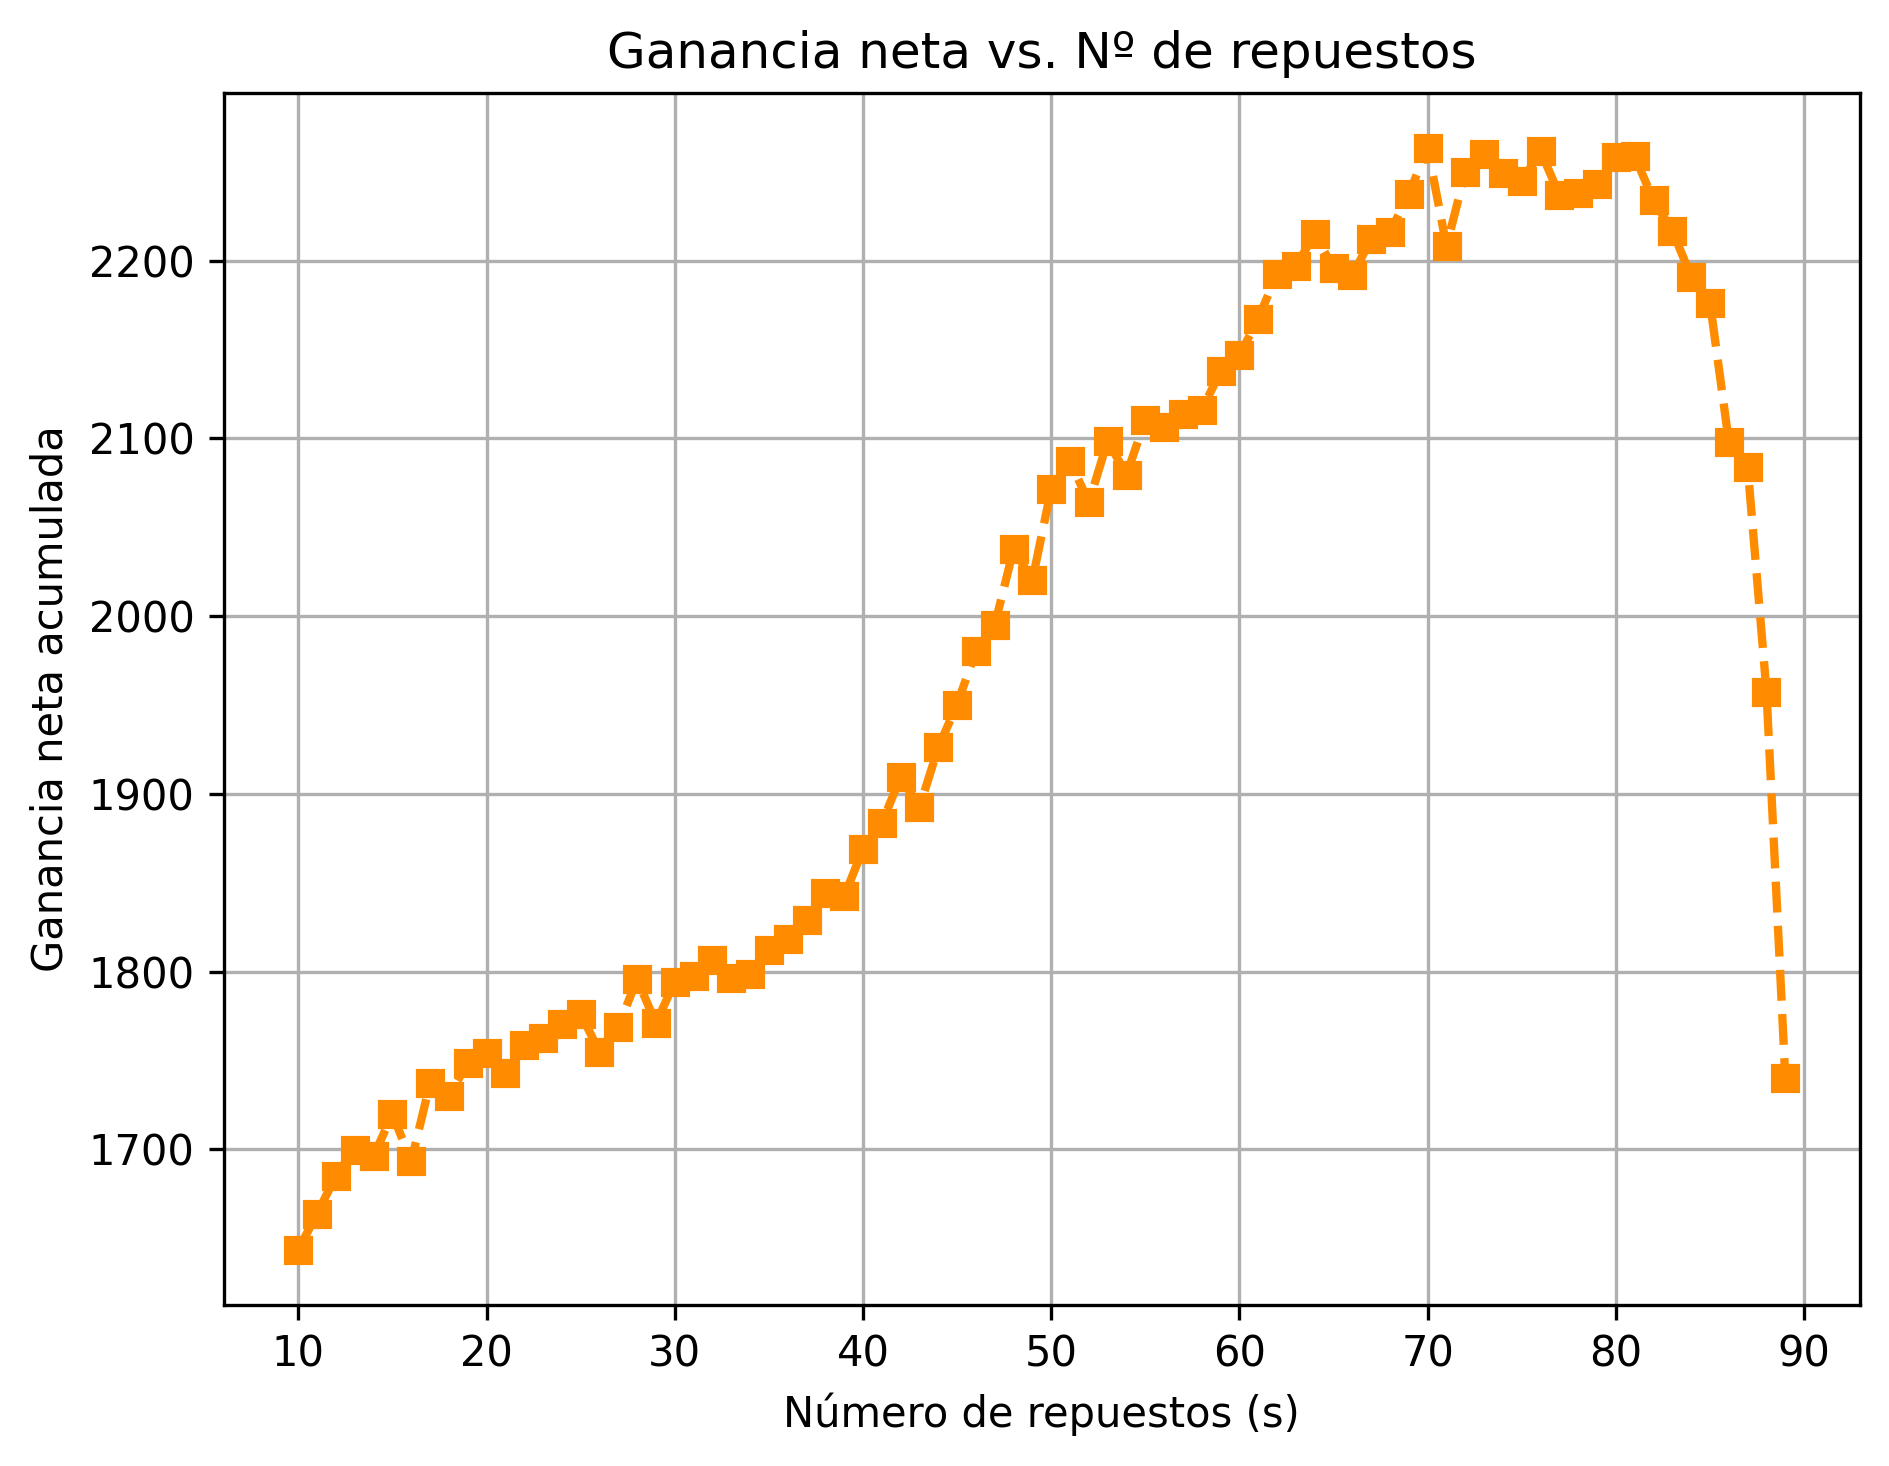
\includegraphics[width=\textwidth]{figure2.png}
			\caption{Tiempo de fallo Vs Ganancia Total}
			\label{fig:Tiempo de fallo Vs Ganancia Total}
		\end{figure}
		
		Resultados experimentales: La ganancia neta acumulada crece al aumentar s hasta alrededor de un intervalo entre 70 y 80. Para s superiores a ese valor la ganancia empieza a decrecer rapidamente.
		\newline
		Se concluye que existe un optimo en el numero de respuestos que maxima la ganancia.
			
	
\end{document}